\paragraph{Demonstration of citation}
Table~\ref{tbl:CitationStyles} shows some different options on how to cite a source. 
The examples are done using the \texttt{biblatex} package.
\begin{center}
\begin{minipage}{\columnwidth}% ensure that there is no page or column break	
	\captionof{table}{\label{tbl:CitationStyles}Some styles to citation}
	\begin{tabular}{lll}
		\hline \\
		Command & 	Output	& Citation \\
		\\
		\hline \\
		\verb! \cite{ref} ! & \cite{Monippally2010} & Bare\\
		\verb! \textcite[page]{ref} ! & \textcite[p. 20]{Monippally2010} & Textual\\
		\verb! \parencite[chapter]{ref} ! & \parencite[chap. 4]{Monippally2010} & Parenthetical\\
		
		\verb! \citeauthor{ref} ! & \citeauthor{Monippally2010} & Name\\
		\verb! \citeyear{ref} ! & \citeyear{Monippally2010} & Year\\
		\hline \\
	\end{tabular}  
\end{minipage}
\end{center}
In his introduction to research methodology writing, \citeauthor{Bouchrika2020} refers to some articles \cite{Bouchrika2020,Choy2014,Holden2004}.

\paragraph{Demonstration of abbreviations}
Define a glossary entry in file \texttt{Acronyms.tex}:
\newline
\verb!\newacronym{utc}{UTC}{Coordinated Universal Time}!
\newline
Use a glossary entry: \verb! \gls{utc} !
\newline
This \LaTeX code \verb*|\gls{utc} is 3 hours behind \gls{adt}.| \\
will produce: \\
\gls{utc} is 3 hours behind \gls{adt}.\\

At the first time usage, the abbreviation is mentioned in brackets.
With the second usage of an abbreviation, the abbreviated term itself is not shown any more:
\gls{utc} is still 3 hours behind \gls{adt}.

\paragraph{Demonstration of a horizontal bar chart}
Fig.~\ref{fig:XBarChart} shows an example of a horizontal bar chart generated with tikzpicture (pgfplots package).

\begin{figure}
	\centering
	\begin{tikzpicture}
		\begin{axis}[xbar,tick align=outside,
			%width=11cm,
			%height=8cm,
			bar width={10pt},
			enlarge y limits=0.13,
			enlarge x limits=false,
			nodes near coords,
			nodes near coords align=horizontal,
			use units,
			xmin=0,
			xmax=60,
			xtick={0,10,...,60},
			x unit=\%,
			xlabel=Reduction in diarrhoea morbidity,
			ytick={1,...,6},
			yticklabels={Hand Washing With Soap, Point-of-use Water Treatment, Sanitation, Hygiene Education, Water Supply, Source Water Treatment}
			]
			\addplot
			[draw=blue,fill=blue!15]
			coordinates
			{(11,1) (25,2) (28,3) (32,4) (39,5) (44,6)};
		\end{axis}
	\end{tikzpicture}
	\caption{\label{fig:XBarChart}Title to a x-bar chart}
\end{figure}

\paragraph{Demonstration of a stacked bar chart}
Fig.~\ref{fig:StackedBarChart} shows an example of a stacked bar chart generated with tikzpicture (pgfplots package).

\begin{figure}
	\centering
	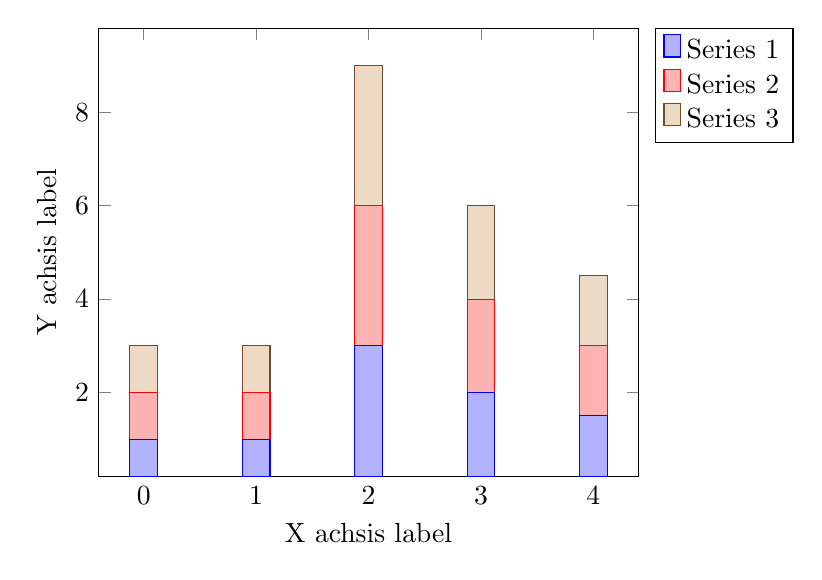
\begin{tikzpicture}
		\begin{axis}[ybar stacked, 
			xlabel=X achsis label, 
			ylabel=Y achsis label,
			legend cell align=left,
			legend pos=outer north east]
			\addplot coordinates 
			{(0,1) (1,1) (2,3) (3,2) (4,1.5)};
			\addplot coordinates
			{(0,1) (1,1) (2,3) (3,2) (4,1.5)};
			\addplot coordinates
			{(0,1) (1,1) (2,3) (3,2) (4,1.5)};
			\legend{Series 1, Series 2, Series 3}
		\end{axis}
	\end{tikzpicture}
	\caption{\label{fig:StackedBarChart}Title to a stacked bar chart}
\end{figure}

\paragraph{Demonstration of a vertical bar chart}
Fig.~\ref{fig:YBarChart} shows an example of a vertical bar chart generated with tikzpicture (pgfplots package).

\begin{figure}
	\centering
	\begin{tikzpicture}
		\begin{axis}[ybar,tick align=outside,
			%width=11cm,
			%height=8cm,
			bar width={10pt},
			enlarge x limits=0.13,
			enlarge y limits=false,
			nodes near coords,
			nodes near coords align=vertical,
			use units,
			ymin=0,
			ymax=100,
			ytick={0,10,...,100},
			y unit=\%,
			ylabel=Response,
			xtick={1,...,7},
			xticklabels={Water for handwashing, Soap for handwashing, Covered pit latrines, Latrines condusive for use, Latrine have doors, Seperate for both boys and girls, Seperate for teachers/pupils},
			x tick label style={rotate=45,anchor=east}
			]
			\addplot
			[draw=blue,fill=blue!15]
			coordinates
			{(1,25) (2,10) (3,5) (4,45) (5,25) (6,100) (7,100)};
		\end{axis}
	\end{tikzpicture}
	\caption{\label{fig:YBarChart}Title to a y-bar chart}
\end{figure}

\paragraph{Demonstration of a clustered bar chart}
Fig.~\ref{fig:ClusteredBarChart} shows an example of a clustered bar chart generated with tikzpicture (pgfplots package).

\begin{figure}
	\centering
	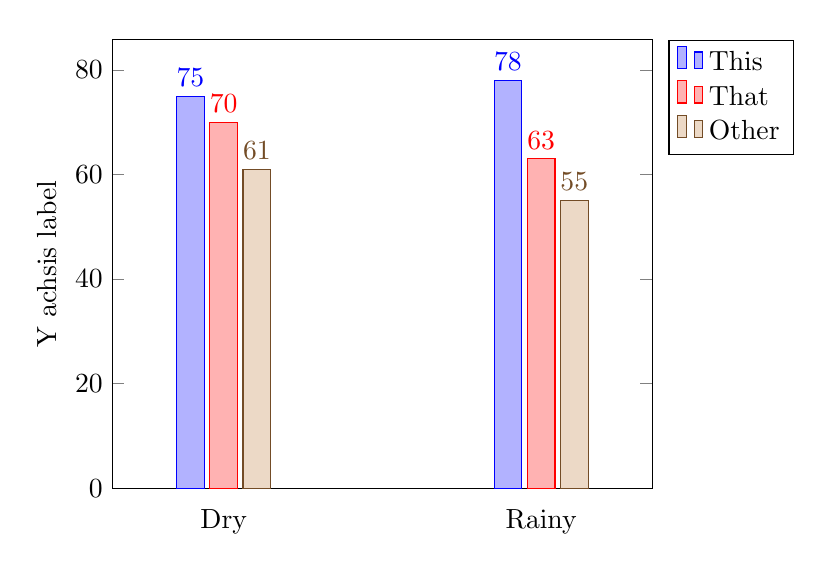
\begin{tikzpicture}
		\begin{axis}  
			[  
			ybar,
			ylabel={Y achsis label}, % there should be no line gap between the rows here. Otherwise, latex will show an error.  
			symbolic x coords={Dry, Rainy},  
			xtick=data,  % groups plots around same tick
			enlarge x limits=0.35, % increases the axis range by 25%
			ymin=0,
			major x tick style = transparent,
			nodes near coords,  
			nodes near coords align={vertical},
			legend cell align=left,
			legend pos=outer north east
			]  
			\addplot coordinates {(Dry, 75) (Rainy, 78)}; % these are the measures of a particular bar graph. The tick marks of the y-axis will be adjusted automatically according to the data values entered in the coordinates.  
			\addplot coordinates {(Dry, 70) (Rainy, 63)};  
			\addplot coordinates {(Dry, 61) (Rainy, 55)};  
			\legend{This, That, Other}  
			
		\end{axis} 
	\end{tikzpicture}
	\caption{\label{fig:ClusteredBarChart}Title to a clustered bar chart}
\end{figure}

\paragraph{Demonstration of a pie chart}
Fig.~\ref{fig:PieChart} shows an example of a pie chart generated with tikzpicture (pgf-pie package).

\begin{figure}
	\centering
	\begin{tikzpicture}
		\pie [rotate = 180]
		{
			62/Category A,
			32/Category B, 
			6/Other
		}
		\end{tikzpicture}
	\caption{\label{fig:PieChart}Title to the pie chart}
\end{figure}

\paragraph{Demonstration of a line chart}
Fig.~\ref{fig:LineChart} shows an example of a simple chart generated with tikzpicture (packages pgfplots and pgfplotstable). 
The regression is also rendered and the formula $ y(x_i) = a \cdot x_i + b$ displayed. The values a and b will be stored globally.

\begin{figure}
	\centering
	\begin{tikzpicture}
		\begin{axis}[legend pos=outer north east]
			\addplot table[row sep=\\] {% plot X versus Y. This is original data.
				X Y\\
				1 1 \\
				2 4\\
				3 9\\
				4 16\\
				5 25\\
				6 36\\
			};
			\addplot table[row sep=\\,
			y={create col/linear regression={y=Y}}] % compute a linear regression from the input table
			{
				X Y\\
				1 1 \\
				2 4\\
				3 9\\
				4 16\\
				5 25\\
				6 36\\
			};
			\addlegendentry{$y(x)$}
			\addlegendentry{%
				$\pgfmathprintnumber{\pgfplotstableregressiona} \cdot x
				\pgfmathprintnumber[print sign]{\pgfplotstableregressionb}$}
		\end{axis}

	\end{tikzpicture}
	\caption{\label{fig:LineChart}Title to the line chart}
\end{figure}

\paragraph{Demonstration of a table}
Table~\ref{tbl:Salinity-EC} shows an example of a table. Different parts of the Final Year Report and their corresponding weights for marking them can be viewed at table~\ref{tbl:ModuleWeight}. A help to generate LaTeX tables can be found at \url{https://www.tablesgenerator.com/}.

\begin{table}% float, LaTeX will move it to whatever position is 'best'
	%\begin{minipage}{\columnwidth}
	\centering
	\captionabove{Conductivity values measured for defined salinity values}
	\label{tbl:Salinity-EC}
	\begin{tabular}{cc}
		\hline \\
		Salinity [g/L]	& 	Electrical Conductivity [mS/cm]\\    
		\\
		\hline \\
		40	&	63,3	\\
		35	&	55,1	\\
		30	&	47,2	\\
		25	&	40,4	\\
		20	&	32,9	\\
		15	&	25,5	\\
		10	&	17,53	\\
		5	&	9,39	\\
		\hline \\
	\end{tabular}  
	%\end{minipage}
\end{table}
	
% No float used here! Will be placed just after the last paragraph 
% Let's hope it fits, if not we'll get some ugly space.
\begin{center}% insert some space before and after the table
	\begin{minipage}{\columnwidth}% ensure that there is no page or column break
	\centering% center the table
	\captionof{table}{Module CIV4202 Final Year Report - Assessment}% captionof must be used instead of \caption outside the figure-environment
	\label{tbl:ModuleWeight}
	\begin{tabular}{llc}
		\hline \\
		Category					& Chapter or Feature				& Weight \\
		\\
		\hline \\
		Engineering Content (60\%)	& Introduction and Objectives		& 10\%   \\
									& Problem definition				& 5\%    \\
									& Literature review					& 5\%    \\
									& Methods							& 15\%   \\
									& Results and Discussion			& 15\%   \\
									& Conclusions and recommendations	& 10\%   \\
		Language (25\%)				& Grammar and spelling				& 15\%   \\
									& Sentence structure				& 10\%   \\
		References (15\%)			& Use of references					& 10\%   \\
									& Quality and format of references	& 5\%    \\
		\hline \\
	\end{tabular}
	\end{minipage}
\end{center}

\paragraph{Demonstration of including a section of a PDF}
Fig.~\ref{fig:GF543kv} shows an example of a PDF. The section displayed is of a particular page from the PDF and is cropped in size.
\begin{figure}
	\centering
	\includegraphics[width=0.7\textwidth,page=6, trim = 25mm 172mm 25mm 45mm, clip]{600-Appendices/Examples/Datasheet_GF_543}
	\caption{GF ball valve 543 kv-characteristic}
	\label{fig:GF543kv}
\end{figure}

\paragraph{Demonstration of including a graphics}
Fig.~\ref{fig:thermometer} shows an image stored as jpg-file. The file is limited to the page width and is rotated by 90\textdegree. Because of the rotation 'height' becomes 'width'.


\begin{center}% insert some space before and after the table
\begin{minipage}{\columnwidth}% ensure that there is no page or column break
	\centering
	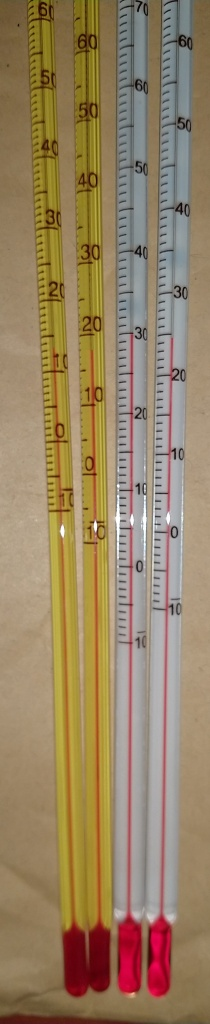
\includegraphics[height=1\textwidth, angle=90]{600-Appendices/Examples/Thermometer.jpg}
	\captionof{figure}{Thermometers showing different temperature readings.} % \captionof instead of \caption because not in figure-environment
	\label{fig:thermometer}	
\end{minipage}
\end{center}

\newpage

\paragraph{Demonstration of including a JPG with labels}
Fig.~\ref{fig:HeatExchanger} shows an example of a JPG that has some labels applied.

\begin{figure}
	\centering
	\label{fig:HeatExchanger}
	\setlength {\unitlength}{0.1\textwidth}
	\begin{picture} (10,7)(0,0)
		\setlength\fboxsep{1 mm}
		\put(0,0){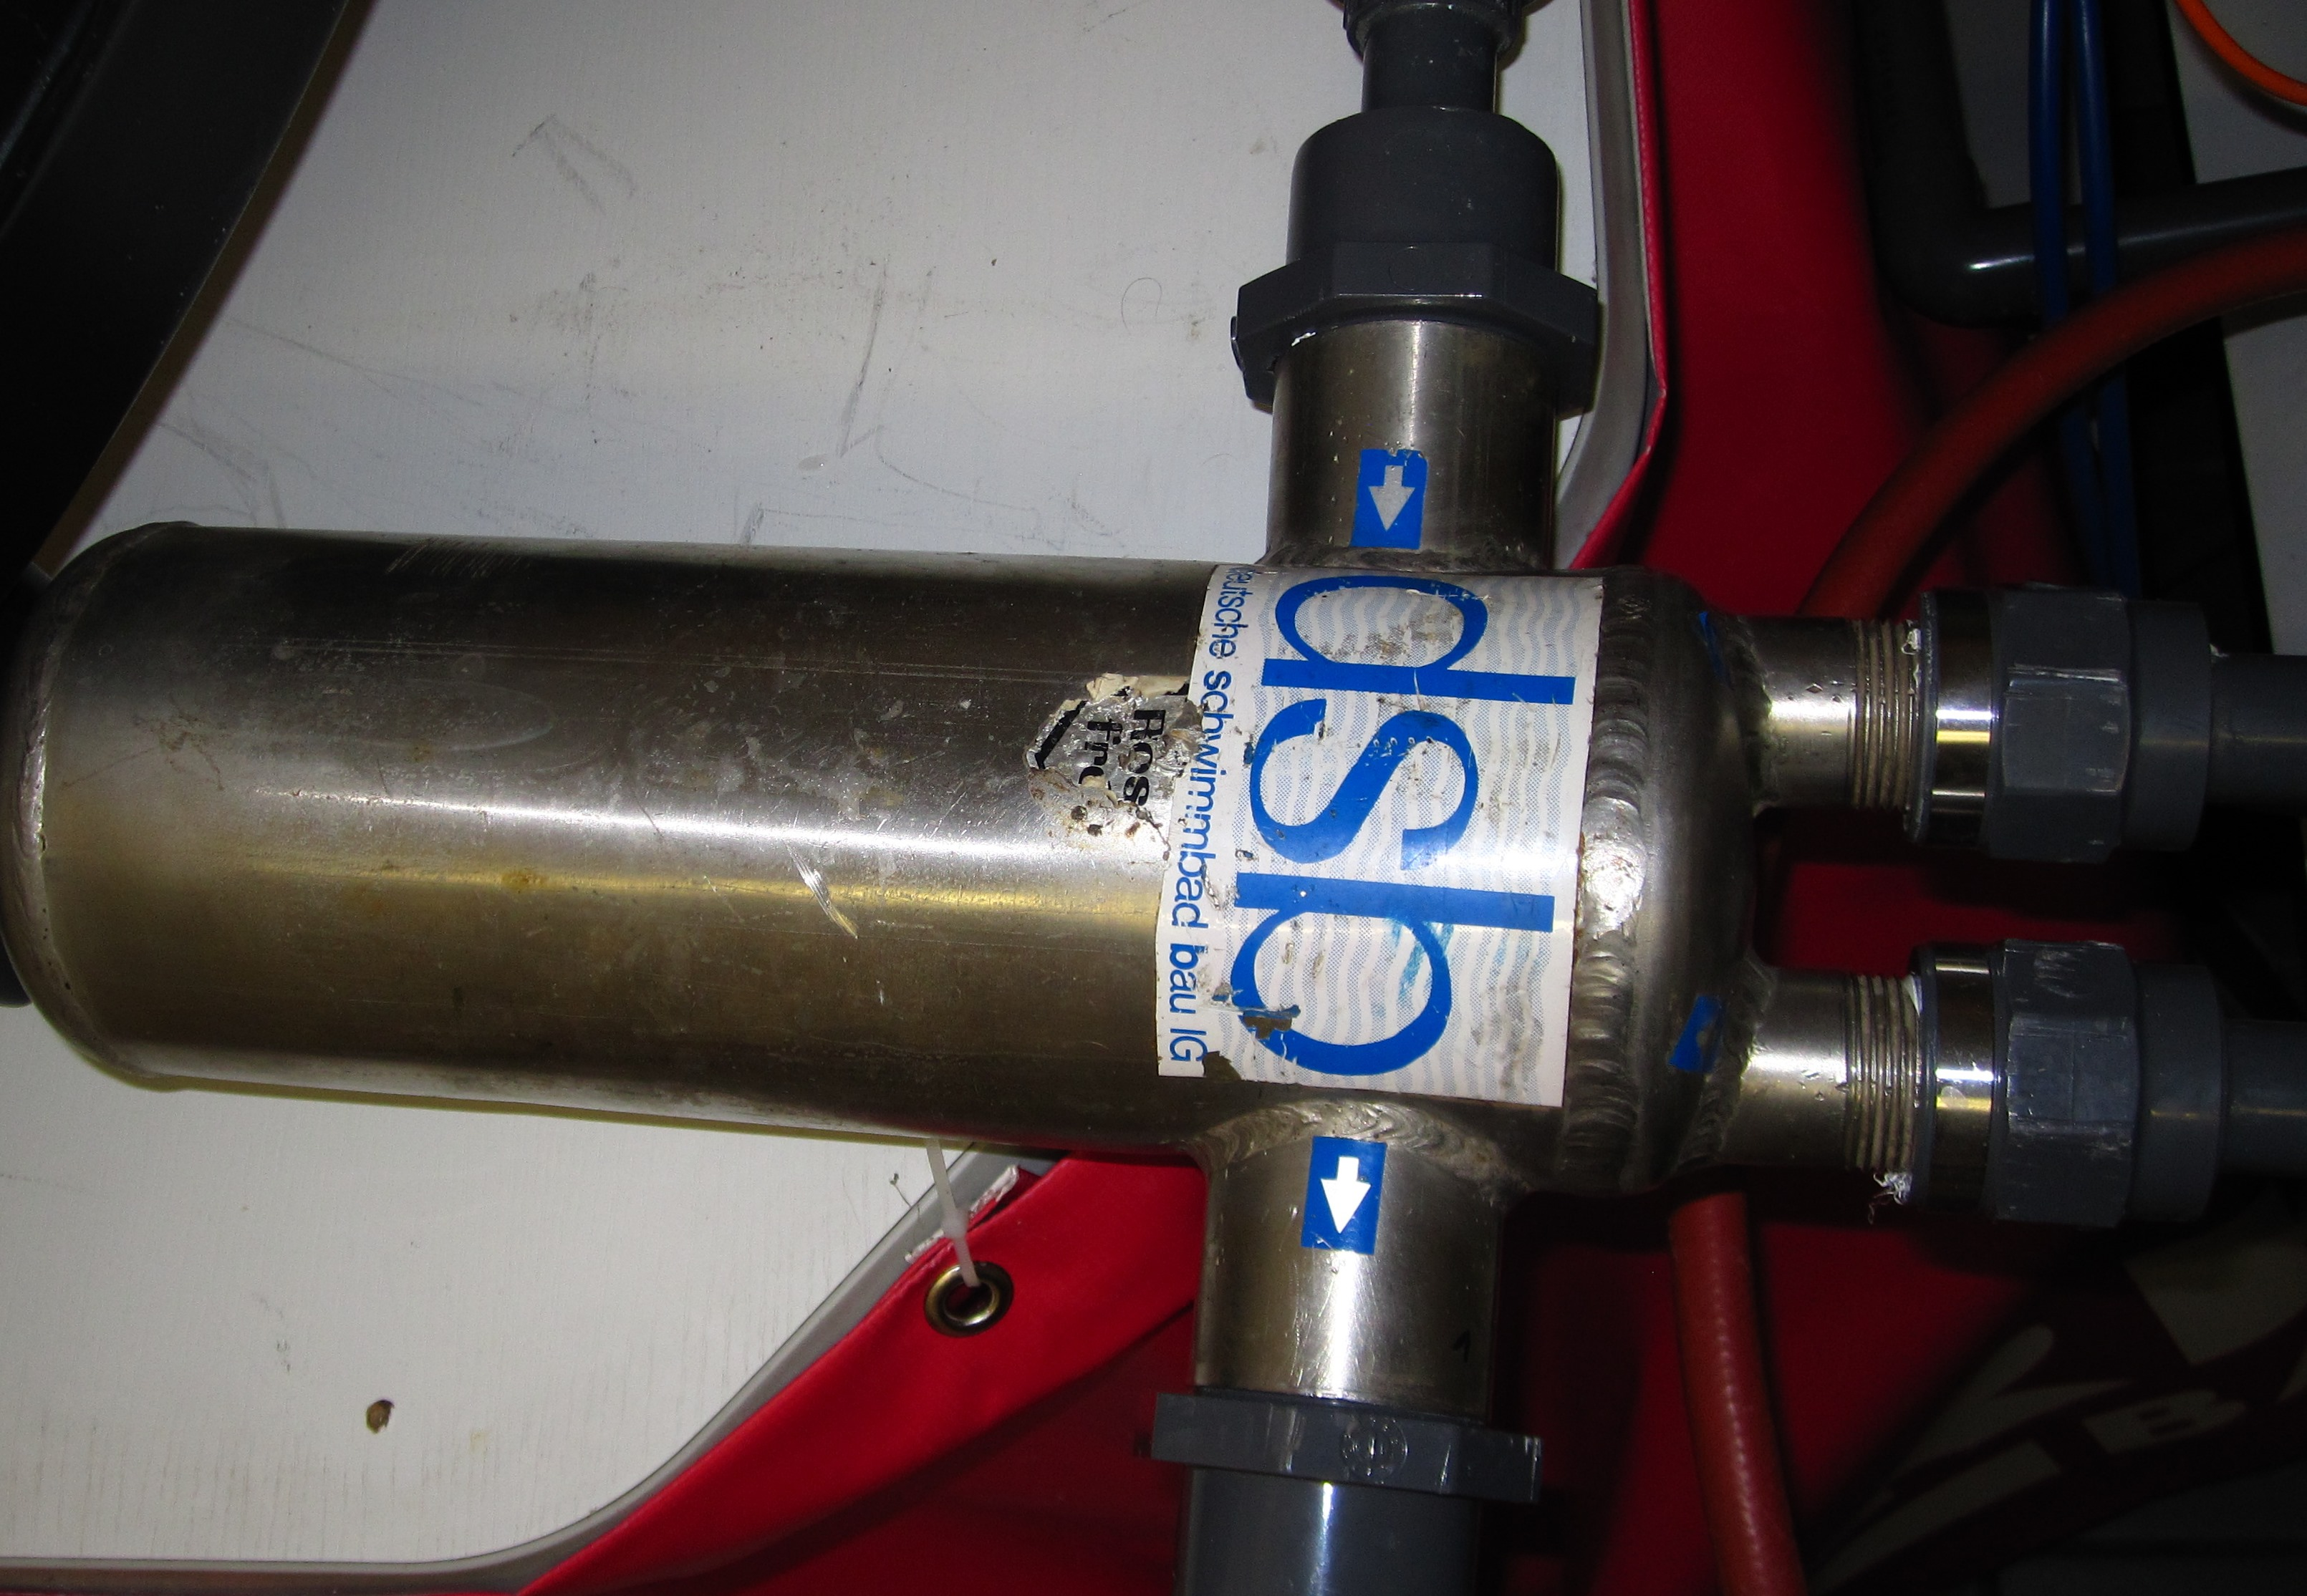
\includegraphics[width=1\textwidth]{600-Appendices/Examples/Heat_Exchanger.jpg}}
		\put(4,5){\colorbox{red!20}{\framebox[1.1\width]{Concentrate in}}}
		\put(3,1){\colorbox{red!20}{\framebox[1.1\width]{Concentrate out}}}
		\put(7,4.5){\colorbox{blue!20}{\framebox[1.1\width]{From exchanger}}}
		\put(7,1.5){\colorbox{blue!20}{\framebox[1.1\width]{To exchanger}}}
	\end{picture}              
	\caption{Heat exchanger with flow of media}
\end{figure}

\paragraph{Demonstration of links}
Use \verb!\href{URL}{DESCRIPTION}! to add a link with description.
Use \verb!\url{URL}! to add a link without a description.
The Water Research \& Development Centre's website: \url{https://nduwrdc.org}\\
Very long urls with hyphens are also possible:\\ \url{http://www.emarketer.com/blog/index.php/quick-stat-smartphone-users-account-38-mobile-phone-users/}

\newpage

\paragraph{Demonstration of equations}
Equation \eqref{equ:Population} shows the geometrical projection formula for population growth.
The parameters description is done using the macro \textit{conditions}, defined at \texttt{NDUmacros.tex}.

\begin{minipage}{\columnwidth}% keep 'equation' and 'conditions' together on same page
	\begin{equation}\label{equ:Population}
	P_f=P_0(1+\frac{i}{100})^t
	\end{equation}
	where:
	\begin{conditions}
		P_f	&	Future population \\
		P_0	&	Current population \\
		i	&	Growth rate in \% \\   
		t	&	Time in years
	\end{conditions}
\end{minipage}

The Hazen-Williams formula expressed in metric units as seen in \eqref{equ:Hazen-William} is used to calculate the headloss.\\

\begin{minipage}{\columnwidth}% keep 'equation' and 'conditions' together on same page
	\begin{equation}\label{equ:Hazen-William}
	H[m]= \Big( \frac{6.78 L}{d^{1.165}} \Big) \Big({\frac{V}{C}} \Big)^{1.85}
	\end{equation}
	where:
	\begin{conditions}
		H	&	Headloss \\
		L	&	Length of pipe\\
		d	&	Internal diameter of pipe \\   
		V	&	Flow \\
		C	&	Coefficient
	\end{conditions}
\end{minipage}

\clearpage

\paragraph{Demonstration of mathematical operations}
It is possible to calculate within \LaTeX{}. In the process, variables can be used to make it easier to modify.
\newcommand\varR{0.6}
\newcommand\varN{0.013}
\newcommand\varS{0.0025}
\newcommand\varResult{\fpeval{round(1/\varN*\varR^(2/3)*\varS^(1/2),3)}}

With values for R=\varR m, n=\varN, S=\varS{}, \eqref{equ:Manning} will result in v=\varResult m/s.\\
The user defined macro \verb! \showcalculation ! (\texttt{NDUmacros.tex}) is also available for calculations:
\showcalculation[\frac{1.0}{\varN} \varR^{2/3} \varS^{1/2}]{round(1/\varN*\varR^(2/3)*\varS^(1/2),3)}

\begin{minipage}{\columnwidth}% keep 'equation' and 'conditions' together on same page
	\begin{equation}\label{equ:Manning}
		v = \frac{1.0}{n} R^{2/3} S^{1/2}	
	\end{equation}
	where:
	\begin{conditions}
		v	&	velocity in m/s\\
		R	&	hydraulic radius in m\\
		n	&	Manning roughness coefficient (dimensionless)\\   
		S	&	slope of the energy grade line (dimensionless)
	\end{conditions}
\end{minipage}

\paragraph{Demonstration of symbols}
In TeXstudio instead of viewing the \textit{Structure} in the side panel, click on $\ast$ to get a list of symbols. Once inserted a leading and trailing \$ must be placed around the symbol code. Some examples displayed using tabbing:
\begin{tabbing}
	\hspace{2in}     			\= \hspace{0.40in}  \= \hspace{1in}    		\kill
	\verb!$\pm$! 				\> $\rightarrow$ 	\> $\pm$ 				\\
	\verb!$\Longrightarrow$! 	\> $\rightarrow$ 	\> $\Longrightarrow$ 	\\
	\verb!$\alpha$! 			\> $\rightarrow$ 	\> $\alpha$ 			\\
	\verb!$\pi$! 				\> $\rightarrow$ 	\> $\pi$ 				\\
	\verb!$\mu$! 				\> $\rightarrow$ 	\> $\mu$	 			\\
\end{tabbing}

\paragraph{Demonstration of flowcharts}
You can follow the instructions of \url{overleaf.com} on creating flowcharts,  \url{https://www.overleaf.com/learn/latex/LaTeX\_Graphics\_using\_TikZ:\_A\_Tutorial\_for\_Beginners\_(Part\_3)\%E2\%80\%94Creating\_Flowcharts}, to achieve Fig.~\ref{fig:flowchart1}~and~\ref{fig:flowchart2}.
\begin{figure}
	\centering
	\begin{tikzpicture}[node distance=2cm]
		\node (start) [startstop] {Something to start with};
		\node (proc1) [process, right of=start, xshift=4cm] {Something else};
		\node (proc2) [process, below of=proc1, yshift=-0.5cm] {
			\begin{minipage}{4cm} %use minipage to have lists
				\begin{itemize}
					\item first item
					\item second item
				\end{itemize}
			\end{minipage}
			};
		\node (proc3) [process, below of=start, yshift=-.5cm] {more here};
		\node (proc4) [process, below of=proc3, xshift=2.5cm, yshift=-0.5cm,  align=left] {many lines\\line 2\\line 3\\line 4}; % align-key needed for \\linebreak 
		\draw [arrow] (start) -- (proc1);
		\draw [arrow] (start) -- (proc3);
		\draw [arrow] (proc1) -- (proc2);
		\draw [arrow] (proc3) -- (proc4);
		\draw [arrow] (proc4) -- (proc2);
	\end{tikzpicture}	
	\caption{Example of a flow chart}
	\label{fig:flowchart1}
\end{figure}

\begin{figure}
	\centering
	\begin{tikzpicture}[node distance=4cm]
		\node (start) [startstop] {Something to start with};
		\node (proc1) [process, right of=start, xshift=0.5cm, yshift=2cm] {A};
		\node (proc2) [process, right of=start, xshift=0.5cm, yshift=-2cm] {B};
		\node (proc3) [process, right of=proc1, yshift=1cm, align=left] {A1\\A1a};
		\node (proc4) [process, right of=proc1, yshift=-1cm, align=left] {A2\\A2b};
		\node (proc5) [process, right of=proc2, yshift=1cm] {B1};
		\node (proc6) [process, right of=proc2, yshift=-1cm] {B2};
		\draw [arrow] (start) -- (proc1);
		\draw [arrow] (start) -- (proc2);
		\draw [arrow] (proc1) -- (proc3);
		\draw [arrow] (proc1) -- (proc4);
		\draw [arrow] (proc2) -- (proc5);
		\draw [arrow] (proc2) -- (proc6);
	\end{tikzpicture}	
	\caption{Some sort of a tree}
	\label{fig:flowchart2}
\end{figure}

\clearpage
\paragraph{Demonstration of a circular diagram}
There is a number of examples using the smartdiagram package here: \url{https://texample.net/tikz/examples/all/}. Fig.~\ref{fig:flowchart3} is one of them.
\begin{figure}
	\centering
	\smartdiagram[circular diagram:clockwise]{ABC, DEF, GHI, JKL, MNO}
	\caption{Circular diagram}
	\label{fig:flowchart3}
\end{figure}

\paragraph{Demonstration of chemical equations and molecules} Package \texttt{mhchem}  provides commands for typesetting chemical molecular formulae and equations:

\schemestart
2 \ce{Mg_{(s)}} + \ce{O2_{(g)}}\arrow{->}2 \ce{MgO_{(s)}} 
\schemestop

\vskip1em
Package \texttt{chemfig} supports the drawing of molecules in 2D and 3D.\\
Here is a reaction with the names under the molecules:

\chemnameinit{\chemfig{R-C(-[:-30]OH)=[:30]O}}
\schemestart
\chemname{\chemfig{R’OH}}{Alcohol}
\+
\chemname{\chemfig{R-C(-[:-30]OH)=[:30]O}}{Carboxylic acid}
\arrow(.mid east--.mid west)
\chemname{\chemfig{R-C(-[:-30]OR’)=[:30]O}}{Ester}
\+
\chemname{\chemfig{H_2O}}{Water}
\schemestop
\chemnameinit{}